\documentclass[13pt,a4paper]{extarticle}
\usepackage[utf8]{inputenc}
\usepackage[utf8]{vietnam} %Bien dich duoc tieng Viet
\usepackage{amsmath,amsfonts,amssymb} %Font toan
\usepackage{type1cm}
\usepackage{times}
\usepackage{graphicx}
\graphicspath{ {images01/} }
\usepackage{enumerate}
\usepackage{comment}
\usepackage{multicol}
\usepackage{multirow}
%\usepackage[unicode]{hyperref} %Tu dong tao bookmark
\usepackage[unicode, hidelinks=true]{hyperref}
\usepackage{indentfirst} %Thut vao dau dong o tat ca cac doan
\usepackage{listings} %Dinh dang code
\usepackage{color} %Mau sac
\usepackage[left=2.5cm,right=2.5cm,top=2.5cm,bottom=2.5cm]{geometry} %Canh lề trái - phải - trên - dưới cho tài liệu
\usepackage{longtable}
\renewcommand{\arraystretch}{1.3}

\begin{document}
\pagenumbering{gobble}
\title{\Large{\textbf{BÁO CÁO THỰC TẬP ĐIỆN CÔNG NGHIỆP}}\\\vspace{1cm}\textbf{Bài 1}\\\vspace{.5cm}\textbf{KHẢO SÁT CẤU TẠO CỦA KHÍ CỤ ĐIỆN}}
\date{Ngày 10 tháng 05 năm 2016}
%\date{\today}
\author{GVHD: Võ Minh Thiện \vspace{.6cm}\\  Nhóm SVTH: Nhóm 2 -- Tiểu nhóm 1: Thi Minh Nhựt}
\maketitle
\tableofcontents
\newpage
\pagenumbering{arabic}
\setcounter{page}{1}
\section{Các khí cụ điện}
\subsection{Khối cầu dao điện E22-KS}
Nguyên lý hoạt động:
\begin{figure}[!h]
\begin{center}
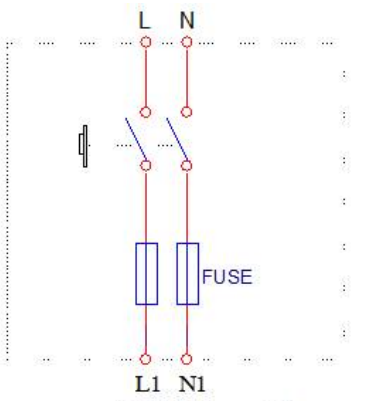
\includegraphics[scale=.5]{cau-dao-dien}
\end{center}
\caption{Khối cầu dao điện}
\end{figure}
\begin{list}{--}{}
\item Dựa vào lưỡi dao và hệ thống kẹp lưỡi mà mạch điện được đóng ngắt.
\item Khi đóng: tiếp điểm động (thân dao) được gắn vào hệ thống kẹp lưỡi $\longrightarrow$ kín mạch.
\item Khi ngắt: tách tiếp điểm động (thân dao) ra khỏi hệ thống kẹp lưỡi $\longrightarrow$ hở mạch.
\item Khi thao tác, cần phải thực hiện nhanh và dứt phát để hạn chế hồ quang.
\end{list}

Ở khối cầu dao người ta thường lắp chung với cầu chì để bảo vệ ngắn mạch, điện áp làm việc của cầu dao đến $660V$.
\subsection{Cầu dao đảo điện E22-TKS}
Nguyên lý hoạt động:
\begin{figure}[!h]
\begin{center}
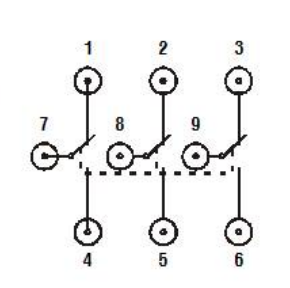
\includegraphics[scale=.7]{cau-dao2-dien}
\end{center}
\caption{Khối cầu dao đảo điện}
\end{figure}
\begin{list}{--}{}
\item Gồm 2 thống tiếp điểm tĩnh cho 2 mạch khác nhau.
\item Đóng mạch 1: ta cho tiếp động (thân dao) gắn vào tiếp điểm tĩnh 1 (hệ thống kẹp lưỡi 1, các tiếp điểm 1, 2, 3) $\longrightarrow$ mạch 1 có điện.
\item Đóng mạch 2: ta cho tiếp động (thân dao) gắn vào tiếp điểm tĩnh 2 (hệ thống kẹp lưỡi 2, các tiếp điểm 4, 5, 6) $\longrightarrow$ mạch 2 có điện.

$\Longrightarrow$ Mạch 1 và mạch 2 không thể cùng có điện.
\item Khi ngắt mạch: tách tiếp điểm động (thân dao) ra khỏi hệ thống kẹp lưỡi 1 hoặc 2 $\longrightarrow$ hở mạch.
\end{list}
\subsection{Công tắc xoay}
Hệ thống tiếp điểm và nguyên lý hoạt động:
\begin{list}{--}{}
\item Khi chưa xoay công tắc, ta gọi:\\
\begin{figure}[!h]
\begin{center}
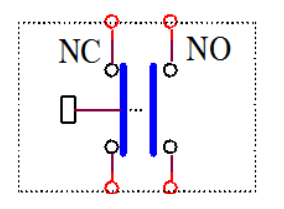
\includegraphics[scale=.7]{nut-nhan-1}
\end{center}
\caption{Công tắc xoay}
\end{figure}
\begin{list}{+}{}
\item Tiếp điểm $1 - 2$: là tiếp điểm thường mở -- $NO$.
\item Tiếp điểm $3 - 4$: là tiếp điểm thường đóng -- $NC$.
\end{list}
\item Khi xoay công tắc: thì các tiếp điểm trên sẽ đổi trạng thái:
\item Tiếp điểm $1 - 2$: tiếp điểm thường mở -- $NO$ $\longrightarrow$ tiếp điểm thường đóng $NO$.
\item Tiếp điểm $3 - 4$: tiếp điểm thường đóng -- $NC$ $\longrightarrow$ tiếp điểm thường mở $NO$.
\end{list}
\newpage
\subsection{Khối nút nhấn PB-2 và PB-3}
\subsubsection{Khối nút nhấn PB-2}
Nguyên lý hoạt động:
\begin{list}{--}{}
\item Khi chưa nhấn nút nhấn:
\begin{list}{+}{}
\item Tiếp điểm OFF: là tiếp điểm thường đóng -- $NC$.
\item Tiếp điểm ON: là tiếp điểm thường mở -- $NO$.
\end{list}
\begin{figure}[!h]
\begin{center}
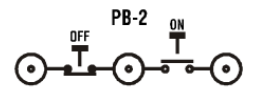
\includegraphics[scale=.7]{nut-nhan-2}
\end{center}
\caption{Nút nhấn PB-2}
\end{figure}
\item Khi nhấn nút nhấn: sẽ đảo ngược trạng thái lại.
\begin{list}{+}{}
\item Tiếp điểm OFF: thường đóng -- $NC$ $\longrightarrow$ thường mở -- $NO$.
\item Tiếp điểm ON: thường mở -- $NO$ $\longrightarrow$ thường đóng -- $NC$.
\end{list}
\item Khi nhả nút nhấn: trở lại trạng thái khi chưa nhấn nút.
\end{list}
\subsubsection{Khối nút nhấn PB-3}
Nguyên lý hoạt động:
\begin{list}{--}{}
\item Khối nút nhấn được tích hợp gồm 3 nút nhấn: STOP, nút FWD, nút REV. 
\begin{figure}[!h]
\begin{center}
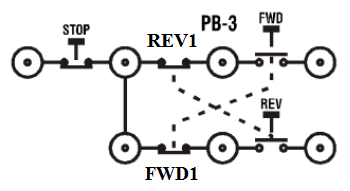
\includegraphics[scale=.7]{nut-nhan-3}
\end{center}
\caption{Nút nhấn PB-3}
\end{figure}
\item Với cách bố trí như trên hình:
\begin{list}{+}{}
\item Khi nhấn nút STOP ngắt mạch hoàn toàn (từ tiếp điểm $NC \longrightarrow NO$).
\item Khi nhấn nút FWD: từ tiếp điểm $NO \longrightarrow NC$, đồng thời tiếp điểm FWD1 từ $NC \longrightarrow NO$.
\item Khi nhấn nút REV: từ tiếp điểm $NO \longrightarrow NC$, đồng thời tiếp điểm REV1 từ $NC \longrightarrow NO$.
\end{list}
\item Ứng dụng của mạch: kết hợp với 2 contactor và relay nhiệt tạo thành bộ khởi động từ kép.
\end{list}
\subsection{Khối relay thời gian E22-TM}
Nguyên lý hoạt động:
\begin{figure}[!h]
\begin{center}
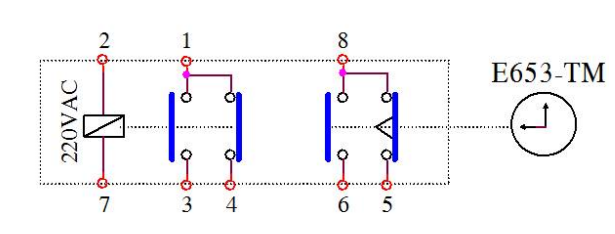
\includegraphics[scale=.7]{relay-timer}
\end{center}
\caption{Relay thời gian}
\end{figure}
\begin{list}{--}{}
\item Khi ta cài đặt thời gian (có thể tắc hoặc mở) qua việc điều chỉnh núm xoay và các giai đo: giờ, phút, giây.
\item Sau thời gian đã cài đặt: có dòng điện chạy qua cuộn dây, sẽ sự thay đổi trạng thái của hệ thống các tiếp điểm: tiếp điểm thường đóng sẽ thành tiếp điểm thường mở và ngược lại, thường mở thành thường đóng.
\end{list}
Thí nghiệm kiểm tra:
\begin{list}{--}{}
\item Cài đặt thời gian cho relay là $5s$.
\item Trước khi cấp nguồn vào cuộn hút: các tiếp điểm  $1-3$ và $6-8$ ở trạng thái thường mở -- $NO$, tiếp điểm $5-8$ ở trạng thái thường đóng -- $NC$.
\item Khi cấp nguồn vào cho cuộn hút: sau 5s, đo lại trạng thái: tiếp điểm $1-3$ và $6-8$ ở trạng thái đóng -- $NC$, còn tiếp điểm $5-8$ thì ở trạng thái mở $NO$.
\item Khi ngắt nguồn điện ra thì trở lại trạng thái khi chưa cấp nguồn cho cuộn hút.
\end{list}
\newpage
\subsection{Khối công tắc bảo vệ dòng rò}
Nguyên lý hoạt động:
\begin{list}{--}{}
\item Hoạt động dựa trên nguyên lý bảo vệ so lệch.
\item Dựa trên sự cân bằng giữa tổng dòng điện đi vào và tổng dòng điện đi ra.
\item Khi thiết bị tiêu thụ bị rò điện, một phần dòng điện sẽ rẽ xuống đất $\Longrightarrow$ là dòng điện rò.
\item Relay so lệnh sẽ phát hiện ra sự mất cân bằng này (có dòng chạy xuống đất) và điều khiển cắt mạch điện nhờ vào thiết bị bảo vệ so lệch.
\end{list}
\subsubsection{Bảo vệ dòng rò một pha}
\begin{figure}[!h]
\begin{center}
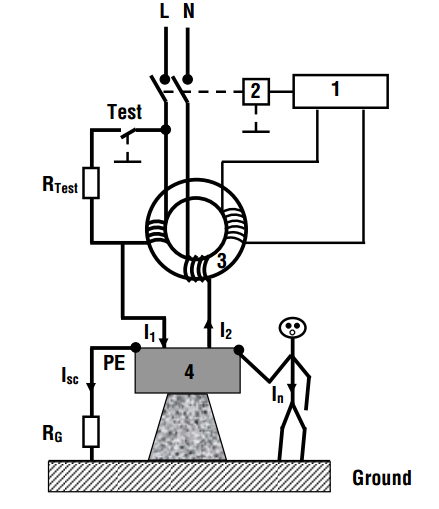
\includegraphics[scale=.7]{cong-tac-bve-ro-1pha.png} 
\end{center}
\caption{Công tắc bảo vệ dòng rò một pha}\label{Fig:RCD1}
\end{figure} 
Phân tích nguyên lý hoạt động dựa trên hình~\ref{Fig:RCD1}:
\begin{list}{--}{}
\item Khi làm việc bình thường: $\vec{I_1} = \vec{I_2}$, kín mạch.
\item Khi có sự cố rò điện: $\vec{I_1} = \vec{I_2} + \vec{I_{sc}}$, thiết bị bảo vệ so lệch sẽ tác động cắt mạch.
\end{list}

Chúng ta có thể kiểm tra bằng cách nhấn nút Test trên thiết bị để tạo sự cố giả, cho thiết bị bảo vệ tác động làm hở mạch.
\subsubsection{Bảo vệ dòng rò ba pha}
\begin{figure}[!h]
\begin{center}
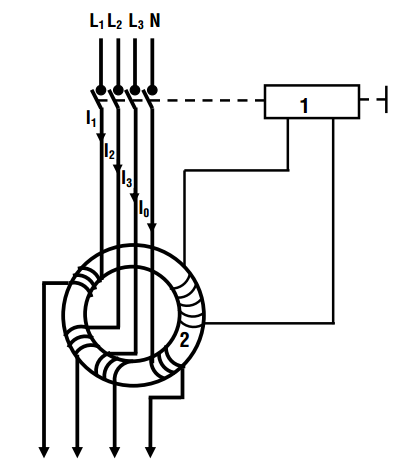
\includegraphics[scale=.7]{cong-tac-bve-ro-3pha.png} 
\end{center}
\caption{Công tắc bảo vệ dòng rò ba pha}\label{Fig:RCD3}
\end{figure}
Phân tích nguyên lý hoạt động dựa trên hình~\ref{Fig:RCD3}:
\begin{list}{--}{}
\item Khi làm việc bình thường: $\vec{I_1} + \vec{I_2} + \vec{I_3} + \vec{I_0} = \vec{0}$, kín mạch.
\item Khi có sự cố rò điện: $\vec{I_1} + \vec{I_2} + \vec{I_3} + \vec{I_0} \neq \vec{0}$, thiết bị bảo vệ so lệch sẽ tác động cắt mạch.
\end{list}

Chúng ta có thể kiểm tra bằng cách nhấn nút Test trên thiết bị để tạo sự cố giả, cho thiết bị bảo vệ tác động làm hở mạch.
\subsection{Contactor ba pha}	
Nguyên lý hoạt động:
\begin{list}{--}{}
\item Khi chưa cấp điện cho cuộn hút:
\begin{list}{+}{}
\item Các tiếp điểm chính là tiếp điểm thường mở.
\item Các tiếp điểm phụ: $NO$ và $NC$.
\end{list}
\item Khi cấp điện cho cuộn hút:
\begin{list}{+}{}
\item Tiếp điểm chính sẽ đóng lại.
\item Đồng thời các tiếp điểm thường $NO$ và $NC$ ban đầu sẽ đổi trạng thái cho nhau: $NC \rightarrow NO$ và $NO \rightarrow NC$.
\end{list}
\end{list}

Thí nghiệm kiểm tra:
\begin{list}{--}{}
\item Mạch khởi động động cơ có tính tự giữ: sử dụng tiếp điểm thường mở $NO$ của contactor.
\begin{figure}[!h]
\begin{center}
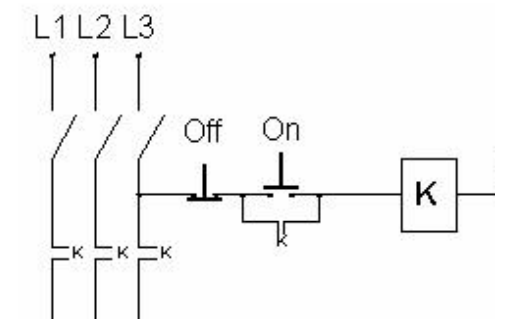
\includegraphics[scale=.55]{contactor-1}
\end{center}
\caption{Mạch có tính tự giữ}
\end{figure}
\begin{list}{+}{}
\item Khi đóng cầu dao 3 pha: nhấn nút $ON$ $\rightarrow$ cuộn hút $K$ có điện.
\item Hệ thống tiếp điểm chính của contactor sẽ đóng lại, cung cấp điện cho tải.
\item Tiếp điểm thường mở $K$ của contactor sẽ đóng lại.
\item Khi nhả nút nhấn ra: dòng điện không còn qua nút $ON$ mà đi qua tiếp điểm $K$, nên cuộn hút có điện liên tục $\rightarrow$ phụ tải phía sau vẫn được cấp điện.
\item Khi nhấn nút $OFF$: hở mạch, cuộn hút $K$ không còn điện, dừng cấp điện cho phụ tải.
\end{list}
\item Mạch khỏi động không tự giữ:
\begin{figure}[!h]
\begin{center}
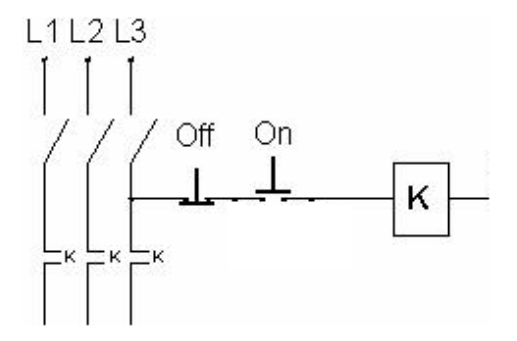
\includegraphics[scale=.55]{contactor-2}
\end{center}
\caption{Mạch không có tính tự giữ}
\end{figure}
\begin{list}{+}{}
\item Trái với mạch có tính tự giữ, mạch không tự giữ cho có điện khi ta còn nhấn nút $ON$.
\item Khi nhả nút $ON$ ra thì cuộn hút $K$ không còn điện $\rightarrow$ hở mạch phía phụ tải.
\end{list}
\end{list}
\subsection{Relay nhiệt}
Nguyên lý hoạt động:
\begin{figure}[!h]
\begin{center}
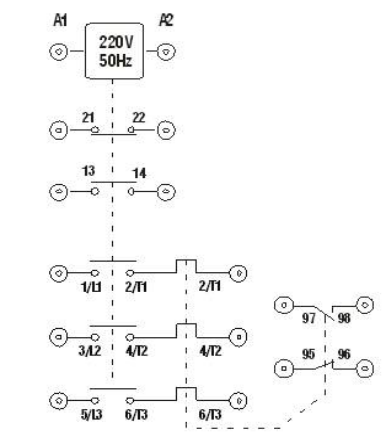
\includegraphics[scale=.7]{relay-temp-1}
\end{center}
\caption{Relay nhiệt kết hợp với contactor}\label{con+relay}
\end{figure}
\begin{list}{--}{}
\item Thường dùng kết hợp với contactor để tạo thành bộ khởi động từ.
\item Ở chế độ vận hành bình thường: phần tử nhạy cảm nhiệt relay nhiệt ở trạng thái đóng, cho phép dòng điện đi qua.
\item Khi động cơ vận hành quá tải, sinh nhiệt vượt quá nhiệt độ cài đặt, phần tử nhạy cảm nhiệt độ sẽ làm cho dòng điện không đi qua bằng cách hở mạch $\rightarrow$ không còn cấp điện cho phụ tải.
\item Như trên hình \ref{con+relay}, khi hoạt động bình thường, tiếp điểm $95-96$ ở trạng thái đóng, khi có sự cố tiếp điểm $95-96$ mở ra để tạo hở mạch, bảo vệ động cơ.
\end{list}
\subsection{Công tắc hành trình E22-PS}
Nguyên lý hoạt động: Về nguyên lý cũng giống như nút nhấn, khi gạt công tắc sẽ có sự thay đổi trạng thái của các tiếp điểm: $NC\rightarrow NO$ và $NO \rightarrow NC$.
\begin{figure}[!h]
\begin{center}
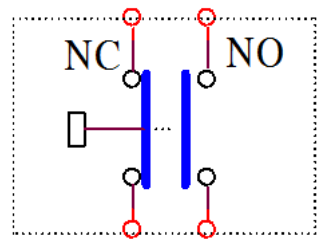
\includegraphics[scale=.6]{nut-nhan-4}
\end{center}
\caption{Công tắc hành trình}
\end{figure}
\newpage
\subsection{Khối cầu chì E653-FS hoặc E653-FU}
Nguyên lý hoạt động:
\begin{list}{--}{}
\item Khi làm việc bình thường: dòng điện chạy qua cầu chì.
\item Khi có sự cố ngắn mạch, quá tải: dòng tăng cao vượt quá dòng định mức của cầu chì, sinh nhiệt lớn, làm đứt dây chảy của cầu chì, gây hở mạch $\longrightarrow$ cách ly sự cố ra khỏi nguồn điện cung cấp.
\end{list}
\subsection{Bộ biến dòng E22-CT}
Nguyên lý hoạt động:
\begin{figure}[!h]
\begin{center}
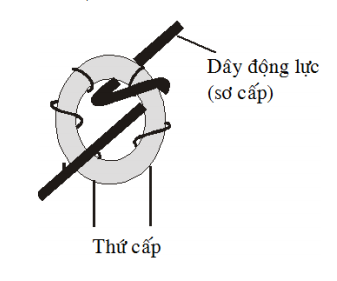
\includegraphics[scale=.7]{bien-dong}
\end{center}
\caption{Khối biến dòng}
\end{figure}
\begin{list}{--}{}
\item Máy biến dòng: biến đổi dòng điện có giá trị lớn thành dòng điện chuẩn phục vụ cho các thiết bị đo lường ($5A;1A$).
\item Làm việc dựa trên nguyên lý cảm ứng điện từ, qua mạch từ lõi thép biến đổi dòng điện lớn sang dòng điện nhỏ, cung cấp cho các phụ tải thứ cấp (các dụng cụ đo lường).
\end{list}
\section{Trả lời câu hỏi}
%\begin{table}[!h]
\begin{center}
\begin{tabular}{|c|p{1.7cm}|p{2cm}|p{5cm}|p{5cm}|}\hline
STT & Khí cụ điện & Hướng sử dụng & Ứng dụng & Khí cụ điện khác \\ \hline
1 & Cầu dao điện & Dân dụng và công nghiệp. & Đóng cắt mạch điện (tạo khoảng cách an toàn trông thấy). &  Cầu dao điện $2P$ $15/20/30/60/100A$ $600V$, $3P~30/60/150/200A ~ 600V$\\ \hline
2 & Cầu dao đảo điện & Dân dụng và công nghiệp. & Chuyển mạch và đóng ngắt mạch. & $2P~30/60/100A ~ 600V$, $3P~60/100A ~ 600V$\\ \hline
3 & Công tắc, nút nhấn & Công nghiệp là chủ yếu, dân dụng & Tạo các nút điều khiển. & \\ \hline
4 & Relay thời gian & Công nghiệp là chủ yếu, dân dụng. & Hẹn giờ đóng, ngắt mạch (lặp lại hoặc không) &  RE11 $0.05s-300h$; RE48; REXL4\\ \hline
5 & Bảo vệ dòng rò & Dân dụng, công nghiệp. & Phát hiện dòng rò, ngắt mạch &  1 pha và 3 pha (4 cực và 3 cực)\\ \hline
6 & Contactor & Dân dụng, công nghiệp. & Điều khiển đóng ngắt mạch điện &  1 pha và 3 pha dùng điện áp kích DC hoặc AC\\ \hline
7 & Relay nhiệt & Công nghiệp là chủ yếu. & Bảo vệ sự cố ngắn mạch và quá tải &  Relay nhiệt bảo vệ (ngắt khi vượt quá nhiệt độ cho phép) hoặc Relay nhiệt điều chỉnh nhiệt độ (theo dõi nhiệt độ thiết bị, ra lệnh điều khiển duy trì nhiệt độ cho phép)\\ \hline
8 & Cầu chì & Dân dụng và công nghiệp. & Bảo vệ sự cố ngắn mạch và quá tải &  Lựa chọn phù hợp các loại cầu chì bảo vệ: cáp và đường dây - L; động cơ và máy cắt - M; linh kiện bán dẫn - M; máy biến áp - $T_r$; cầu chì cao áp và cầu chì hạ áp\\ \hline
9 & Biến dòng & Công nghiệp. & Biến đổi dòng điện lớn về dòng điện do lường &  Các loại biến dòng đưa về dòng đo lường chuẩn là $5A$ và $1A$\\ \hline
\end{tabular}
\end{center}
\end{document}